% =============================================================================
\section{Cooperative states}
% =============================================================================

A Bell inequality sets a limit on observable correlations in a physical system that obeys a local hidden variable theory (\abbrev{lhv})~\cite{Bell1964,Clauser1969}.
This is a classical theory where the results of the measurements are functions of local detector settings and a hidden parameter $\lambda$.
Thus, values measured by two spatially separated observers, $A$ and $B$ (for Alice and Bob, as they are usually denoted), can be expressed as $A(a, \lambda)$ and $B(b, \lambda)$, where $a$ and $b$ are Alice's and Bob's detector settings.
Possible correlations are defined probabilistically as
\begin{eqn}
\label{eqn:bell-ineq:cooperative:lhv}
    C(A,B)
    = \int_{\Lambda} A(a, \lambda) B(b, \lambda) P(\lambda) \upd\lambda.
\end{eqn}
Experimental values $A$ and $B$ are usually encoded as either $1$ or $-1$ in a binary experiment.
The Bell theorem derives inequalities that any such correlations in a \abbrev{lhv} theory must satisfy.
Quantum mechanics violates these inequalities, thus ruling out \abbrev{lhv} theories.


% =============================================================================
\subsection{Quantum state}
% =============================================================================

In this section we will consider Bell violations in cooperative states with $N$ photon pairs, similar to those demonstrated experimentally by Clauser~\cite{Clauser1969}, Aspect \textit{et~al}~\cite{Aspect1982}, and Zeilinger \textit{et~al}~\cite{Weihs1998}.
The quantum state in question is
\begin{eqn}
\label{eqn:bell-ineq:cooperative:state}
    \vert N \rangle
    = \frac{%
        \left(
            \hat{a}_{1+}^{\dagger} \hat{a}_{2+}^{\dagger}
            + \hat{a}_{1-}^{\dagger} \hat{a}_{2-}^{\dagger}
        \right)^{N} \vert 0 \rangle%
        }{N! \left( N+1 \right)^{1/2}},
\end{eqn}
where $N$ is the number of photon pairs, indices $1$ and $2$ denote the propagation direction, and $+$ and $-$ stand for the polarization direction.
These states are generated in certain types of optical parametric down-conversion experiments, and it has proved difficult to obtain a direct, loophole free violation of a Bell inequality, owing to detector inefficiencies~\cite{Cabello2007,Larsson1998,Larsson2001} (although this problem has been solved recently~\cite{Giustina2013}).
However, these issues are not significant for the simulations in this thesis since we are considering an ideal experiment.

We define the intensity correlations to be~\cite{Drummond1983}
\begin{eqn}
\label{eqn:bell-ineq:cooperative:G}
    G^{IJ}(\gamma,N)
    = \langle N \vert
        \hat{A}^{I}(1,\hat{\avec}_{1})
        \hat{A}^{J}(\gamma,\hat{\avec}_{2})
        \vert N \rangle,
\end{eqn}
where $\gamma$ is a linear combination parameter related to the polarizer angle, and auxiliary functions are introduced so that:
\begin{eqn}
    \hat{A}^{J}(\gamma,\hat{\avec}_{k})
    ={} & \left(
            \sqrt{\gamma} \hat{a}_{k-}^{\dagger}
            + \sqrt{1-\gamma} \hat{a}_{k+}^{\dagger}
        \right)^{J}
        \left(
            \sqrt{\gamma} \hat{a}_{k-}
            + \sqrt{1-\gamma} \hat{a}_{k+}
        \right)^{J}, \\
    \hat{A}^{J}(\infty,\hat{\avec}_{k})
    ={} & :\left(
        \hat{a}_{k-}^{\dagger} \hat{a}_{k-}
        + \hat{a}_{k+}^{\dagger}\hat{a}_{k+}
        \right)^{J}: .
\end{eqn}

For $N$ photon pairs, the Bell-type inequality is then known to be of the form~\cite{Drummond1983}
\begin{eqn}
\label{eqn:bell-ineq:cooperative:violation}
    \Delta_N^J(\theta) = 3g_N^J(\theta) - g_N^J(3\theta) - 2 \le 0,
\end{eqn}
where
\begin{eqn}
    g_{N}^{J}(\theta) = G^{JJ}(\cos^{2}\theta,N) / G^{JJ}(\infty,N).
\end{eqn}
This expression generalizes the usual Clauser, Horne, Shimony and Holt (\abbrev{chsh})~\cite{Clauser1969} and Bell expressions to a multi-particle form.
The quantum mechanical prediction for $g_{N}^{J}$ has especially simple form of $g_{N}^{N}(\theta)=\cos^{2N}\theta$ for the cases $J=N$, $N=1,2$ which we have simulated.
This gives the violation of
\begin{eqn}
\label{eqn:bell-ineq:cooperative:violation-1}
    \Delta_{\mathrm{1\, pair}}(\theta)
    \equiv \Delta_1^1(\theta)
    = 3\cos^{2}\theta - \cos^{2}3\theta - 2
\end{eqn}
for the two-particle case, which corresponds to the usual two-particle experiment originally proposed by Bell.
For the four-particle case, the violation can be found to be
\begin{eqn}
\label{eqn:bell-ineq:cooperative:violation-2}
    \Delta_{\mathrm{2\, pairs}}(\theta)
    \equiv \Delta_2^2(\theta)
    = 3\cos^{4}\theta - \cos^{4}3\theta - 2.
\end{eqn}


% =============================================================================
\subsection{Positive-P representation}
% =============================================================================

We simulate the violation~\eqnref{bell-ineq:cooperative:violation} using the positive-P representation~\cite{Drummond1980,Gardiner2004}.
In essence, it is an exact expansion of an arbitrary density matrix of bosons with a positive probability distribution $P(\balpha, \bbeta)$, such that the expectation of an observable $\hat{O}$ is
\begin{eqn}
\label{eqn:bell-ineq:cooperative:pos-P-expectation}
    \langle \hat{O} \rangle
    = \int \upd^2 \balpha\, \upd^2 \bbeta\,
        P(\balpha,\bbeta)
        \langle \bbeta^* \vert \hat{O} \vert \balpha \rangle /
        \langle \bbeta^* \vert \balpha \rangle,
\end{eqn}
where $\vert\balpha\rangle$ is a multimode coherent state.
The positive P-representation, therefore, corresponds exactly to the definition of a physical weak measurement~\cite{Aharonov1988}, with the initial state $\vert\balpha\rangle$ and the final postselected state $\vert\bbeta\rangle$ occurring with probability $P(\balpha,\bbeta)$.
The standard form we use is also known to be measurable using multiple beam-splitter operations~\cite{Agarwal1994}.

The expression above looks very similar to~\eqnref{bell-ineq:cooperative:lhv}, given by an \abbrev{lhv} theory.
The fundamental difference, which allows the correlations obtained from the positive-P distribution to violate Bell inequalities, is that the quantities being sampled can be complex numbers of any magnitude.
Only after the weighted averaging with the probability distribution $P$ do they give the value of the observable.

For an arbitrary moment of creation and annihilation operators $\hat{O}(\avec^\dagger, \avec)$, the expectation is calculated as
\begin{eqn}
\label{eqn:bell-ineq:cooperative:moment-expectation}
    \langle \hat{O} \rangle
    = \int \upd^2 \balpha\, \upd^2 \bbeta\,
        P(\balpha,\bbeta)
        O(\bbeta, \balpha),
\end{eqn}
where $O$ is a function produced as a result of replacing any $\hat{a}_i$ with $\alpha_i$ and $\hat{a}_i^\dagger$ with $\beta_i$ in $\hat{O}$.
For example, the mode population $\langle \hat{a}_i^\dagger \hat{a}_i \rangle$ corresponds to the moment $\beta_i \alpha_i$, which is, in general, complex, and only its expectation is real.

The quantum state~\eqnref{bell-ineq:cooperative:state} we are interested in corresponds to the positive-P distribution~\cite{Drummond1983}
\begin{eqn}
\label{eqn:bell-ineq:cooperative:pos-P}
    P(\balpha,\bbeta)
    ={} & \left\{
        \frac{ |
            (\beta_{1+} + \alpha_{1+}^{*}) (\beta_{2+} + \alpha_{2+}^{*})
            + (\beta_{1-} + \alpha_{1-}^{*}) (\beta_{2-} + \alpha_{2-}^{*}) |^{2N}}{%
            (2\pi)^{8} (N+1) (N!)^{2}2^{4N}}
        \right\} \\
        & \times \exp \left(
            -\frac{ |\balpha|^{2} + |\bbeta|^{2}}{2}
        \right).
\end{eqn}
This distribution exists and has a positive, probabilistic behavior for all values of $N$.
Note that it is not unique, and it may be possible to find other expressions that correspond to the same quantum state, but have better sampling properties.


% =============================================================================
\subsection{Sampling}
% =============================================================================

In order to illustrate our point better, we simulate the measurement of the operator~\eqnref{bell-ineq:cooperative:G} using the Monte-Carlo method: we sample the distribution~\eqnref{bell-ineq:cooperative:pos-P} and calculate the weighted average~\eqnref{bell-ineq:cooperative:pos-P-expectation}.

We sample this distribution by transforming it to a form where we can use the well-known von Neumann rejection algorithm.
Performing the variable change
\begin{eqn}
\label{eqn:bell-ineq:cooperative:mu-lambda}
    \bmu = \frac{\balpha - \bbeta^*}{2},\quad
    \blambda = \frac{\balpha + \bbeta^*}{2},
\end{eqn}
and grouping the components of $\blambda$ and $\bmu$ as
\begin{eqn}
\label{eqn:bell-ineq:cooperative:ab-delta-ab}
    \Avec & = [ \lambda_{1+}, \lambda_{1-} ],\quad
    \Bvec = [ \lambda_{2+}, \lambda_{2-} ],\\
    \delta\Avec & = [ \mu_{1+}, \mu_{1-} ],\quad
    \delta\Bvec = [ \mu_{2+}, \mu_{2-} ],
\end{eqn}
we can separate the positive-P function into independent parts as
\begin{eqn}
    P(\Avec, \Bvec, \delta\Avec, \delta\Bvec)
    = P^\prime(\Avec, \Bvec) G(\delta\Avec) G(\delta\Bvec).
\end{eqn}
Here $G$ is a $4$-component Gaussian distribution with the variance $\sigma^2 = 1/2$ in each real component
\begin{eqn}
    G(\delta\Avec)
    = \frac{1}{\pi^2} e^{-|\delta\Avec|^2},
\end{eqn}
and $P^\prime$ is the distribution core with a reduced number of variables
\begin{eqn}
    P^\prime(\Avec, \Bvec)
    = \left(
            \frac{ |\Avec \cdot \Bvec |^{2N} }{\pi^4 (N+1) (N!)^2}
        \right)
        e^{-|\Avec|^2 - |\Bvec|^2},
\end{eqn}

The Gaussian parts can be sampled exactly using conventional methods, while the distribution core requires requires an application of rejection sampling.
Since $|\Avec\cdot\Bvec| \le |\Avec| |\Bvec|$, $P^\prime$ can be bounded as
\begin{eqn}
    P^\prime(\Avec, \Bvec) \le F(\Avec) F(\Bvec),
\end{eqn}
where
\begin{eqn}
    F(\Avec)
    = \frac{|\Avec|^2N}{\pi^2 \sqrt{N+1} N!} e^{-|\Avec|^2}.
\end{eqn}
The bounding function $F$ will be used as a probability distribution in the rejection sampling, so it must be normalised on $1$.
In order to do this, we notice that
\begin{eqn}
    \int |\Avec|^{2N} e^{-|\Avec|^{2}} \upd^2 \Avec
    & = S_{k-1}(1) \int_0^{\infty} r^{2N+k-1} \exp(-r^{2}) \upd r \\
    & = \frac{1}{2} \Gamma(N+k/2) S_{k-1}(1),
\end{eqn}
where $k$ is the number of components in $\Avec$ (in our case $\Avec$ contains two complex numbers, so $k=4$), and $S_{k-1}(R)$ is the surface area of a $k$-dimensional ball:
\begin{eqn}
    S_{k-1}(r) = \frac{2\pi^{k/2} r^{k-1}}{\Gamma(k/2)}.
\end{eqn}
Thus, the normalisation coefficient is
\begin{eqn}
    M
    = \int F(\Avec) \upd^2 \Avec
    = \frac{\Gamma(N+2)}{2\pi^{2}\sqrt{N+1}N!} \times \frac{2\pi^{2}}{\Gamma(2)}
    = \sqrt{N+1},
\end{eqn}
and $F(\Avec) = M F^\prime(\Avec)$, where $F^\prime$ is a probability distribution
\begin{eqn}
    F^\prime(\Avec)
    = \frac{|\Avec|^{2N}}{\pi^2 (N+1)!} e^{-|\Avec|^2}.
\end{eqn}

The distribution $F^\prime$, in turn, can be represented as a product of two independent distributions~\cite{Gupta1997}:
\begin{eqn}
    F^\prime(\Avec)
    \equiv F^\prime(r,\nvec)
    = S_{k-1}(r) g(r^2) U(\nvec)
    = R(r) U(\nvec),
\end{eqn}
where $r = |\Avec|$, $\nvec$ is a unit vector on a $k$-dimensional sphere, and $U=1/S_{k-1}(1)$ is a uniform distribution of vector directions (or, in other words, a uniform distribution on the surface of a $k$-dimensional ball).
The latter can be sampled using the Marsaglia algorithm~\cite{Marsaglia1972} (sampling a vector of $k$ normally distributed random numbers and normalising it on $1$).
In order to sample the distribution $R$, we have to make another variable change, $r^{2}\rightarrow x$:
\begin{eqn}
    R(x)
    & = \frac{1}{2\sqrt{x}} S_{k-1}(\sqrt{x}) g(x) \\
    & = \frac{1}{2\sqrt{x}}
        \frac{2\pi^{k/2} x^{(k-1)/2}}{\Gamma(k/2)}
        \frac{x^{N}}{\pi^2 (N+1)!} e^{-x} \\
    & = \frac{x^{N+1}}{(N+1)!} e^{-x}.
\end{eqn}
The result is exactly the gamma-distribution with the scale $\alpha = N + 2$, for which an efficient sampling method exists~\cite{Marsaglia2000}.

In summary, the rejection algorithm for sampling the probability distribution~\eqnref{bell-ineq:cooperative:pos-P} consists of the following steps:
\begin{enumerate}
\item Sample two squared lengths $|\Avec|^2$ and $|\Bvec|^2$ using the gamma distribution with the scale $N+2$.
\item Sample two directions $\nvec_A$ and $\nvec_B$ using the Marsaglia algorithm.
\item Combine squared lengths and directions into $\Avec$ and $\Bvec$.
\item Sample $u$ from the uniform distribution on $[0,1)$.
\item If $u > P^\prime(\Avec,\Bvec) / (M^2 F^\prime(\Avec) F^\prime(\Bvec))$, reject the sample and start over.
\item Sample the real components of $\delta\Avec$ and $\delta\Bvec$ independently using Gaussian distributions with the variance $1/2$ and combine them with $\Avec$ and $\Bvec$ to get $\balpha$ and $\bbeta$ using~\eqnref{bell-ineq:cooperative:ab-delta-ab} and~\eqnref{bell-ineq:cooperative:mu-lambda}.
\end{enumerate}
The resulting phase-space coordinates $\balpha$ and $\bbeta$ can be now used to obtain a sample of any moment of creation and annihilation operators using the formula~\eqnref{bell-ineq:cooperative:moment-expectation}.


% =============================================================================
\subsection{Results}
% =============================================================================

\begin{figure}
    \centerline{%
    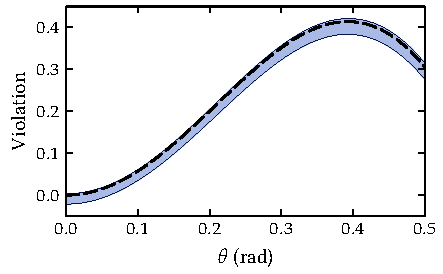
\includegraphics{figures_generated/bell/cooperative_N1.pdf}%
    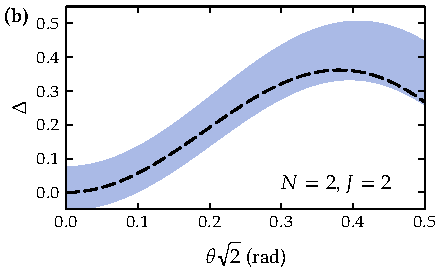
\includegraphics{figures_generated/bell/cooperative_N2.pdf}}

    \caption[Simulated Bell violation for cooperative states]{
    Simulated Bell violation $\Delta_N^J$ as a function of the relative polarizer angle $\theta$ for \textbf{(a)} one, and \textbf{(b)} two photon pairs using the positive-P distribution with \textbf{(a)} $2^{21}$ and \textbf{(b)} $2^{25}$ samples.
    The filled area corresponds to the estimated sampling error around the mean of $\Delta_N^J(\theta)$ for the sampled state, while the dashed line is the exact quantum mechanical prediction of this value.}%endcaption

    \label{fig:bell-ineq:cooperative:violation}
\end{figure}

Using the sampling method described in the previous subsection, we can now sample the positive-P distribution~\eqnref{bell-ineq:cooperative:pos-P} and calculate the violation~\eqnref{bell-ineq:cooperative:violation}.
We do this for the two-particle case $N=J=1$, and also for the four-particle case $N=J=2$, which has also been observed experimentally~\cite{Howell2002}.
The results are plotted in~\figref{bell-ineq:cooperative:violation}, together with the analytical predictions~\eqnref{bell-ineq:cooperative:violation-1} and~\eqnref{bell-ineq:cooperative:violation-2}.
The second case requires significantly more samples to achieve a small enough sampling error, but it is clear that in both cases we were able to demonstrate a violation which is beyond the sampling error range.
This is a direct counterexample to Feynman's claim.
